% `template.tex', a bare-bones example employing the AIAA class.
%
% For a more advanced example that makes use of several third-party
% LaTeX packages, see `advanced_example.tex', but please read the
% Known Problems section of the users manual first.
%
% Typical processing for PostScript (PS) output:
%
%  latex template
%  latex template   (repeat as needed to resolve references)
%
%  xdvi template    (onscreen draft display)
%  dvips template   (postscript)
%  gv template.ps   (onscreen display)
%  lpr template.ps  (hardcopy)
%
% With the above, only Encapsulated PostScript (EPS) images can be used.
%
% Typical processing for Portable Document Format (PDF) output:
%
%  pdflatex template
%  pdflatex template      (repeat as needed to resolve references)
%
%  acroread template.pdf  (onscreen display)
%
% If you have EPS figures, you will need to use the epstopdf script
% to convert them to PDF because PDF is a limmited subset of EPS.
% pdflatex accepts a variety of other image formats such as JPG, TIF,
% PNG, and so forth -- check the documentation for your version.
%
% If you do *not* specify suffixes when using the graphicx package's
% \includegraphics command, latex and pdflatex will automatically select
% the appropriate figure format from those available.  This allows you
% to produce PS and PDF output from the same LaTeX source file.
%
% To generate a large format (e.g., 11"x17") PostScript copy for editing
% purposes, use
%
%  dvips -x 1467 -O -0.65in,0.85in -t tabloid template
%
% For further details and support, read the Users Manual, aiaa.pdf.


% Try to reduce the number of latex support calls from people who
% don't read the included documentation.
%
\typeout{}\typeout{If latex fails to find aiaa-tc, read the README file!}
%


\documentclass[]{aiaa-tc}% insert '[draft]' option to show overfull boxes

 \title{Celestial Navigation Device for Future Autonomous Applications}

 \author{
 Thomas Fuller%
    \thanks{Graduate Researcher, Mechanical Engineering, University of New Hampshire, 33 Academic Way, Durham, NH, 03824},
    \
 William Nitsch%
    \thanks{Graduate Researcher, Electrical Engineering, University of New Hampshire, 33 Academic Way, Durham, NH, 03824},
  \ and May-Win Thein%
    \thanks{Associate Professor, Mechanical Engineering, University of New Hampshire, 33 Academic Way, Durham, NH, 03824}
  %\thanksibid{1}
  \\
  {\normalsize\itshape}\\
  %\and
  %Third C. Author%
  % \thanks{Job Title, Department, Address, and AIAA Member Grade.}\\
  %{\normalsize\itshape
  %Business or Academic Affiliation, City, Province, Zipcode, Country}
 }

 % Data used by 'handcarry' option if invoked
 %\AIAApapernumber{16-509}
 %\AIAAconference{Spaceflight Mechanics Conference, Feb. 2016, Napa, CA}
 %\AIAAcopyright{\AIAAcopyrightD{2016}}

 % Define commands to assure consistent treatment throughout document
 \newcommand{\eqnref}[1]{(\ref{#1})}
 \newcommand{\class}[1]{\texttt{#1}}
 \newcommand{\package}[1]{\texttt{#1}}
 \newcommand{\file}[1]{\texttt{#1}}
 \newcommand{\BibTeX}{\textsc{Bib}\TeX}

\usepackage{bm}
\usepackage{amsmath}
\usepackage{subfigure}
%\usepackage[notref,notcite]{showkeys}  % use this to temporarily show labels
\usepackage[colorlinks=true, pdfstartview=FitV, linkcolor=black, citecolor= black, urlcolor= black]{hyperref}
\usepackage{overcite}
\usepackage{footnpag}			      	% make footnote symbols restart on each page
%\usepackage{chngcntr}
%\counterwithout{figure}{section}
%\counterwithout{figure}{subsection}
\begin{document}
\maketitle

\begin{abstract}
Determination of an extraterrestrial rover's latitude and longitude will be an essential part of the exploration of other planets.  This paper presents a self contained, Digital Single Lens Reflex (DSLR) camera based celestial navigation device that is based on nautical Sight Reduction techniques. This paper discusses a novel method for observing the altitude angle of a star. Also presented are simulation results for two different categories of observations, three stars sighted simultaneously and a single star sighted at three different times.  Simulation parameters are derived using measurement uncertainty analysis with both published and experimental values of uncertainty.  Experimental results suggest that a navigational error of approximately 4.5 nautical miles is possible and are presented along with a discussions and analysis on possible improvements.  
\end{abstract}

%\section*{Nomenclature}
%\begin{tabbing}
%  XXX \= \kill% this line sets tab stop
%  $A$ \> Attitude Matrix \\
%  $B$ \> Body Frame\\
%  $I$ \> Inertial Frame \\
%  $G$ \> Greenwich Frame \\
%  $L$ \> Local Frame \\
%  $\lambda$ \> longitude \\
%  $\epsilon$ \> heading \\
%  $\phi^{'}$ \> Compliment of Latitude \\
%  $\phi$ \> Latitude \\
%  $LHA$ \> Local Hour Angle \\
%  $GHA$ \> Greenwich Hour Angle \\
%  $Long$ \> Estimated Longitude \\
%  $\lambda$ \> Estimated Latitude  \\
%  $H_{c}$ \> Computed Altitude \\
%  $Lat$ \> Estimate of Latitude
%  $X,A$ \> Azimuth Parameters
%  $\lambda$ \> longitude
%  
%  $\Delta x$ \> Variable displacement vector \\
%  $\alpha$ \> Acceleration, m/s\textsuperscript{2} \\[5pt]
%  \textit{Subscript}\\
%  $i$ \> Variable number \\
% \end{tabbing}

\section{Introduction}
% probably talk to mw about htis...
%One problem of interest at the University of New Hampshire's Advanced Controls Lab (ACL) is extraterrestrial surface navigation. One vision ACL has is a complete Guidance, Navigation, and Control (GNC), solution for use on the surface of other planets.  The proposed solution focuses on a distributed control scheme that uses a group of differential drive rovers, referred to as a TankBot.  These rovers are generically referred to as mobility solutions.  In the area of Guidance, work presented by M. Johnson in (whatever) covers the use of Particle Swarm Optimization (PSO) and Path Planning.  PSO is one scheme to search an area on the extraterrestrial surface using a large group of robots.  A paper presented in 2012 by Underwood in (whatever) compared the performance of Proportional-Integral-Derivative (PID), Linear-Quadratic-Regulator (LQR), $H_{\infty}$, Sliding Mode Control (SMC), and Fuzzy-LQR controllers.  Underwood concluded that $H_{\infty}$ and SMC were the best candidates for controlling the mobility solution.  Perkins produced results in (whatever) that demonstrated the use of different observation techniques, including Sliding Mode Observer (SMO), Extended Kalman Filter (EKF), and $H_{\infty}$ filter.  Additionally, Perkins performed Monte Carlo simulations that demonstrated the mathematical viability of a matrix formulated celestial navigation algorithm.  This algorithm is the Compass Star Tracker originally proposed by Swanzy et. al in (whatever). The compass star tracker was shown by Texas A\&M University to be a viable method for static position determination. One restriction of CST is that it must be zenith oriented.  It will be demonstrated that the implemented method for eliminating the zenith requirement   This paper presents the algorithms, simulation, and experimental setup for a static positioned, computer vision based celestial navigation device that is self contained and increases the range of angles the device can be held at for meaningful star altitude measurement.
A desirable goal for robotic extraterrestrial surface navigation is autonomous navigation.  Johnson and Thein examined a distributed control scheme intended for extraterrestrial search. \cite{b:johnson}.  Underwood and Thein compared the performance of Proportional-Integral-Derivative (PID), Linear-Quadratic-Regulator (LQR), $H_{\infty}$, Sliding Mode Control (SMC), and Fuzzy-LQR controllers \cite{b:underwood}.  It was concluded that $H_{\infty}$ and SMC were the best candidates for controlling the mobility solution.  Perkins and Thein demonstrated the use of different observation techniques, including Sliding Mode Observer (SMO), Extended Kalman Filter (EKF), and $H_{\infty}$ filter\cite{b:perkins}.  Additionally, Perkins performed Monte Carlo simulations that demonstrated the mathematical viability of a matrix formulated celestial navigation algorithm.  This algorithm is the Compass Star Tracker (CST) originally proposed by Swanzy et. al\cite{b:swanzy}. CST was shown to be a viable method for static position determination. One restriction of CST is that it must be zenith oriented.  It will be demonstrated that the implemented method for eliminating the zenith requirement breaks down at certain pitch and roll angles.  This paper presents the algorithms, simulation, and experimental setup for a static positioned, computer vision based celestial navigation device that is self contained and increases the range of angles the device can be held at for meaningful navigational output.
One method of position determination includes the use of the NASA/ESA Deep Space Network (DSN).  DSN uses light from a quasar in conjunction with three ground stations located in Barstow California, Madrid, Spain, and Canberra, Australia\cite{b:dsn}. DSN is extremely accurate, leading to position error circles between 5 and 10 meters\cite{b:msla}. The primary limitations of DSN are that it has geometric weakness in the southern declinations and that it requires a precisely timed interaction between the ground station, a quasar and the mobility solution\cite{b:dor}.
\section{Celestial Navigation Algorithms}
\subsection*{Compass Star Tracker Method} 
For CST, a Charge Coupled Device (CCD) sensor is used to detect light from the stars.  The star locations are mapped to pixels on the sensor by a centroiding algorithm.  Once the stars have been located on the image, the Pyramid Lost In Space Algorithm (Pyramid-LISA) is invoked.  This algorithm compares the interstar angles for stars on the CCD\cite{b:lisa}.  After this, CST determines the attitude between four reference frames.  The reference frames are B, I, G and L.  This corresponds to body, inertial (geocentric) reference frame, Greenwich reference frame and local reference frame, respectively.  The local reference frame is aligned to the local zenith direction in this derivation. The B frame is an offset to the L frame.  The abridged equation is shown in the below in Eq.~(\ref{fuck}).

\begin{equation}
 \label{fuck}
 A^{B/I}A^{I/G} = A^{B/L}A^{L/G}
\end{equation}
The resulting attitude transformation matrix is given below
\begin{equation}
 \label{fuck}
A^{B/L}A^{L/G} =
    \begin{pmatrix}
    C_{\epsilon}C_{\phi^{'}}C_{\lambda} - S_{\epsilon}S_{\lambda} &
    C_{\epsilon}C_{\phi^{'}}S_{\lambda} + S_{\epsilon}C_{\lambda} &
    -C_{\epsilon}S_{\phi^{'}}\\
    -S_{\epsilon}C_{\phi^{'}}C_{\lambda} - C_{\epsilon}S_{\lambda}&
    -S_{\epsilon}C_{\phi^{'}}S_{\lambda} + C_{\epsilon}C_{\lambda}&
    -S_{\epsilon}S_{\phi^{'}} \\
    S_{\phi^{'}}C_{\lambda} & S_{\phi^{'}}S_{\lambda} & C_{\phi^{'}}
    \end{pmatrix}
\end{equation}
Where $C_{x}$ is defined as $cos(x)$ and $S_{x}$ is defined as $sin(x)$.  The longitude $\lambda$, the heading $\epsilon$, and the compliment of the latitude $\phi^{'}$, can be extracted by using the following equations.  

\begin{equation}
 \label{e:lambdaa}
    \lambda = arctan2[A(3,2), A(3,1)]
\end{equation}
\begin{equation}
 \label{e:epsilonn}
    \epsilon = arctan2[A(2,3), -A(1,3)]
\end{equation}
\begin{equation}
 \label{e:phii}
    \phi^{'} = arcsin[\frac{A(3,2)}{sin\lambda}]
\end{equation}
The latitude can be found from

\begin{equation}
 \label{e:phi}
    \phi = 90 - \phi^{'}
\end{equation}
This derivation for the algorithm has a zenith requirement\cite{b:gpsapps}. Here, we examine this requirement in greater detail. The solution to eliminating the zenith requirement was originally presented by Swanzy and is reiterated below:
\subsection*{Failure Conditions for Zenith Requirement Solution}
One proposed solution for the zenith requirement of CST is derived by Swanzy.  It can be demonstrated that the z component of CST optical axis can be defined in Eq.~(\ref{e:oavector}).  In this equation, $\psi$ and $\xi$ represent the roll and pitch angles, respectively, of the camera body.  
\begin{equation}
 \label{e:oavector}
    \overrightarrow{oa} =
    \begin{bmatrix} 
    sin(\psi) & sin(\xi) & \sqrt{1-sin^{2}(\psi)-sin^{2}(\xi)}
    \end{bmatrix}
\end{equation}
Eq.~(\ref{e:oavector}) has a failure condition.  As $sin^{2}(\psi)+sin^{2}(\xi)$ approaches $1$, the third term of the vector enters the complex domain.  This suggests that the solution does not produce valid results for useful angles of pitch and roll. Combinations of pitch and roll angles that follow this condition can be seen in Fig.~\ref{f:failure}.
It can be seen from the experimental verification of the CST that the orientation angle of the the CST from the vertical never varied by more than approximately 2 degrees. This shows that although CST was not pointed at full zenith, it did not appear to have a wide range of motion.  A table depicting the pointing angles of CST is shown in Fig~\ref{f:alt}.

The inflexibility of the zenith requirement, along with the apparent failure condition of the equation that removes the zenith requirement from CST led to the development of a new algorithm, based on maritime techniques.  \\

\subsection*{Directly Computed Sight Reduction Method}
The proposed method is a computer vision based method that uses the Direct Computation Method for Nautical Sight Reduction \cite{b:naut}.  This method measures the angle between the horizon and star.  This angle is known as the altitude.  The algorithm begins with an estimation of the initial position of the mobility solution. The local hour angle is computed as
\begin{equation}
 \label{e:LHA}
    LHA = GHA + Long
\end{equation}
$H_{c}$ is the altitude of the observed star if the estimated position was the true location.  $H_{c}$ can be calculated as follows.

\begin{equation}
 \label{e:Hc}
    H_{c} = sin^{-1}(Ssin(Lat) - Ccos(Lat))
\end{equation}
In equation~(\ref{e:Hc}), S is defined as $S = sin(Dec)$ and C is defined as $C = cos(Dec)cos(LHA)$.
X, and A are parameters which are used to determine the azimuth direction, and are calculated as follows.
\begin{equation}
 \label{e:X}
    X = \frac{Scos(Lat) - Csin(Lat)}{cos(H_{c})}
\end{equation}

\begin{equation}
 \label{e:A}
    A = cos^{-1}(X)
\end{equation}
In Eq.~(\ref{e:A}), if $LHA > 180^{\circ}$, then set Z = A.  Otherwise, $Z = 360^{\circ} -A$.  The next portion of the sight reduction method is an iterative method which calculates ground distance between the estimated point from $H_c$ and the observed point found with $H_{o}$, known as $p$. $p$ is also referred to as the intercept Eq.~(\ref{e:p}).

\begin{equation}
 \label{e:p}
    p = H_{o} - H_{c}
\end{equation}
\subsection{Center Pixel Method}
Calculation of $H_{o}$ is performed by assigning IMU pitch and roll values to the image center pixel. The Blind Astrometric Calibration of Arbitrarily Astronomical image processing algorithm is used to obtain the altitude angle in the star image\cite{b:astrometry}. This is shown in Eq.~(\ref{e:cpm1}) where the variables are in units of pixels.
\begin{equation}
    \label{e:cpm1}
       \begin{pmatrix} 
  x_{T}     \\ 
  y_{T} 
\end{pmatrix}=\begin{pmatrix} 
  cos(\theta)     & -sin(\theta)\\ 
  sin(\theta) & cos(\theta) 
\end{pmatrix}\begin{pmatrix} 
  x\\ 
  y_{c} + y_{off} 
\end{pmatrix}
\end{equation}
Now that $Z$ and $p$ for each observation are calculated, the terms from the iterative method can be calculated. The terms of each summation are used to calculate the center of the error polygon used for navigation.  Note that $n$ represents the number of iterations.  These terms are listed below.  

\begin{equation}
A = \sum \limits_{i=1}^n cos^{2}Z_{i}
\end{equation}
\begin{equation}
B = \sum \limits_{i=1}^n cosZ_{i}sinZ_{i}
\end{equation}
\begin{equation}
C = \sum \limits_{i=1}^n sin^{2}Z_{i}
\end{equation}
\begin{equation}
D = \sum \limits_{i=1}^n p_{i}cosZ_{i}
\end{equation}
\begin{equation}
E = \sum \limits_{i=1}^n p_{i}sinZ_{i}
\end{equation}
These terms can then be combined as follows.  
\begin{equation}
 \label{e:G}
    G = AC-B^{2}
\end{equation}

\begin{equation}
 \label{e:Bi}
    B_{i} = B_{F} + \frac{CD-BE}{G}
\end{equation}

\begin{equation}
 \label{e:Li}
    L_{i} = L_{f} + \frac{AE - BD}{Gcos(B_{F})}
\end{equation}

\begin{equation}
 \label{e:d}
    d = 60\sqrt{(L_{I} - L_{F})^{2}cos^{2}(B_{F}) + (B_{I} - B_{F})^{2}}
\end{equation}
%In Eq. In Eq.~(\ref{e:Bi}), and Eq.~(\ref{e:Li}), the subscript "I" refers to an "improved" guess, and the subscript "F" refers to a an initial guess.  
The algorithm is repeated until the value of Eq.~(\ref{e:d}) is sufficiently small.  

\subsection*{Measurement Uncertainty Modeling}
The uncertainty of a function, q, in multiple variables, $x, x_{1}, x_{2} ... x_{n}$ is determined by the Pythagorean sum of its partial derivatives multiplied by their respective uncertainties $\Delta x, \Delta x_{1}, \Delta x_{2} ... \Delta x_{n}$\cite{b:error}.  

\begin{equation}
    \label{e:uncertain}
\Delta q = \sqrt{\left(\sum\limits_{i=1}^n  \frac{\partial q}{\partial x_{i}}\Delta x_{i} \right)^{2} }
\end{equation}
\\\\
Eq.~(\ref{e:uncertain}) was used in order to determine the uncertainty for the celestial navigation process.  A roll correction was derived.  This correction rolled the image coordinates $x^{'}, y^{'}$ by an angle $\theta$.  This two dimensional rotation matrix is described in Eq.~(\ref{e:roll})
\begin{equation}
    \label{e:roll}
   \begin{pmatrix} 
  x     \\ 
  y 
\end{pmatrix}=\begin{pmatrix} 
  cos(\theta)     & -sin(\theta)\\ 
  sin(\theta) & cos(\theta) 
\end{pmatrix}\begin{pmatrix} 
  x^{'}\\ 
  y^{'} 
\end{pmatrix}
\end{equation}
Using Eq.~(\ref{e:uncertain}) normalized to determine the fractional uncertainty, the uncertainty for Eq.~(\ref{e:roll}), can be computed to be the following. 

\begin{equation}
\Delta y = \Delta x = \sqrt{\left(\Delta x^{'}\right)^{2} + \left(\Delta y^{'}\right)^{2} + \left(\Delta \theta\right)^{2}}
\end{equation}
This leads to the full uncertainty equation below.
\begin{equation}
    \label{e:sumdelta}
\Delta H_{o} = \sqrt{\left2(\Delta x^{'}\right)^{2} + \left2(\Delta y^{'}\right)^{2} + \left2(\Delta \theta\right)^{2} + \left(\Delta \phi\right)^{2} }
\end{equation}
\section{Simulation}
Simulations were written to demonstrate the use of the nautical sight reduction method.  These simulations also show convergence and accuracy of two different observation formats.  The first observation type is a single star sighted three different times.  The second observation type uses three stars from the same image. A third format using three stars at three different times was tested for convergence only.  
\subsection*{Convergence}
The first test of each observation format is a whether or not Eq.~(\ref{e:d}) converges to a single value.  The algorithm was tested over ten iterations with no additional noise or bias. In Figure~\ref{f:converge} it can be seen that in general the different observational methods converge by the second iteration. Note that all figures can be found in the appendix.  Sighting a single star three times takes four iterations to converge.  This suggests that method may be suboptimal for navigation.
\subsection*{Test of Observational Formats}
Each of the observational formats were tested for their accuracy and ease of implementation with the experimental setup.  Figures~\ref{f:1s3t},~\ref{f:1s3t_hist},~\ref{f:3s1t}, and~\ref{f:3s1t_hist} show the simulated position estimates and corresponding histograms for the celestial navigation device with $\pm 1^{\circ}$ in the estimation of $H_{o}$. The mean value was not an accurate predictor of location when one star was observed three times.  In addition, for points where the randomly generated bias in $H_{o}$ was high, the algorithm sometimes produced non-convergent results.   While observing three stars at the same time, non-convergent values did not appear with the simulated noise threshold.  For this observation format, the mean was an accurate predictor of location.  For these reasons, the experimental celestial navigation device observes three stars at the same time.  
\subsection*{Simulation of Uncertainty}
Approximate values for the uncertainty of the celestial navigation device are based on Eq.~(\ref{e:uncertain}) are given here.  $\Delta x^{'} = \Delta y = 12.1^{'}$ arcseconds.  $\Delta \theta = \Delta \phi = 360$ arcseconds.  Using these values, $\Delta H_{o} = 600$ arcseconds of uncertainty.  $H_{o}$ was computed accounting for significant digits in the uncertainty of the experimental setup. The simulation setting is for three different stars in the field of view being photographed at the same time. 
Figure~\ref{f:crush} shows the distribution of the location estimates with an uncertainty of 600 arcseconds.  
One thousand points were randomly generated using the biases described in Eq.~(\ref{e:sumdelta}). The normal distribution of these estimates suggests that the mean is a good approximation of the true points.
\section{Experiment}
\subsection*{Set Up}
The experimental device is a Nikon D60 DSLR camera, with an attached Nikon 50mm f/1.8D Auto Focus Nikkor Lens.  The lens is set to the "$\infty$" focus setting.  A standard photography tripod is used to stabilize the camera housing along with a remote shutter to prevent movement when the photograph of the stars is taken.  To ensure that adequate light is captured for star identification, the shutter remains open for 8 seconds per photograph. 
A flash attachment houses a Razor 9DOF inertial measurement unit (IMU).  The IMU reports the Euler angles between the local coordinate frame and the camera optical axis frame.  The IMU sets the Euler angles for the center pixel of the camera image.  Since useful navigational stars appear in locations other than the center pixel, an offset from the center pixel is applied using the field of view of the camera lens.  The camera setup has a field of view across the sensor diagonal of approximately 30.5 degrees.  This corresponds to an angular offset of approximately 24.2 arcseconds per pixel away from the center pixel.  An image of the experimental setup can be seen below.  These values for the field of view are calculated automatically in the Astrometry.net package and can also be calculated from $FOV = 2 atan(y_{1}/f)$\cite{b:aov}.  This yields a field of view of 31.707 degrees for the D60.  The camera crop factor reduces the FOV to 30.5 degrees. A laptop is used to record the local time and the IMU Euler angle output. The setup is pictured in Figure~\ref{f:setup}.
\subsection*{Experimental Results}
The same algorithm was performed on experimental images.  Using Astrometry, altitude measurements of star centers were obtained.  These measurements were taken from Durham, New Hampshire.  With no correction for roll, the mean estimated point was 78.2927W, 44.2405N.  The true point was 70.9349W, 43.1337N.  This led to a mean error of 382.9 nautical miles, and can be seen in Figure~\ref{f:nomods}.
A modification of the pitch measurement based on calibration images was added in order to help obtain a more accurate result.  This modification is designed to be close to the unmodeled pitch bias.  The calibration  method attempted to observe a star in the image center pixel and compare $H_{o}$ and $H_{c}$ to determine the bias values. The pitch offset value was -5.159 degrees. The negative sign corresponds to the IMU being pitched too high. The mean estimated point was 71.239W, 44.392N.  The mean error was 77.09 nautical miles.  Error was observed in the latitude as time goes on.  This can be seen in Figure~\ref{f:pitchmod}.
A roll modification improved the accuracy of the estimate.  For a roll error correction of 2 degrees, the following coordinate was obtained: (70.9404W, 43.2087N).  This is a mean error of about 4.5088 nautical miles.  This suggests that correction can be added to the measurements that models the lumped error of the pitch and roll measurements (i.e. misalignment errors to give a more accurate position estimate).  The plot of the roll error correction can be seen in Fig.~\ref{f:zrollmod}.
%It can be seen in figure~\ref{f:setup} that magnetization is a
%function of applied field.


%\begin{table}% no placement specified: defaults to here, top, bottom, page
% \begin{center}
%  \caption{Variable and Fixed Coefficient Runge-Kutta Schemes as a
%           Function of Reynolds Number}
%  \label{t:scheme_comparison}
%  \begin{tabular}{rrr}
%       Re & Vary & Fixed \\\hline
%        1 &  868 & 4,271 \\
%       10 &  422 & 2,736 \\
%       25 &  252 & 1,374 \\
%       50 &  151 &   736 \\
%      100 &  110 &   387 \\
%      500 &   85 &   136 \\
%    1,000 &   77 &   117 \\
%    5,000 &   81 &    98 \\
%   10,000 &   82 &    99
%  \end{tabular}
% \end{center}
%\end{table}
\section{Future Work}
The most important future work will be field testing the celestial navigation device in various locations in order to determine whether or not dynamic navigation is possible with this device.  Current tests were performed in a single location.

Accuracy would be improved by applying the gnomonic projection correction to the image processing suite.  The gnomonic coordinate transformation is essential because the light from the star passes through a spherical lens, onto a CCD element, a flat plane\cite{b:gnomonic}.  %The relationship between the spherical and planar coordinate frames is given as follows.  $\phi_{lens}$ represents the "latitude", and $\lambda_{lens}$ represents the "longitude" coordinate on the lens.
%\begin{equation}
%\phi = sin^{-1} \left ( cos(c)sin(\phi_{1} + \frac{ysin(c)cos(\phi_{1})}{\rho}\right)
%\end{equation}
%
%\begin{equation}
%\lambda = \lambda_{0} + tan^{-1}\left (\frac{xsin(c)}{\rho cos(\phi_{1}) cos(c) - y sin(\phi_{1})sin(c)}\right)
%\end{equation}
%\begin{equation}
%\rho = \sqrt{x^{2} + y^{2}}
%\end{equation}
%\begin{equation}
%c = tan^{-1}(\rho)
%\end{equation}
Without these projections, the experiment will only be valid for an area in the middle of the camera's field of view where the small angle theorem is valid.
\section{Conclusion}  The zenith requirement from the matrix formulated celestial navigation algorithm was shown to be invalid at certain roll and pitch angles.  It was decided that a new algorithm would be developed for celestial navigation on an extraterrestrial mobility solution.  The method of Blind Astrometric Calibration was applied to images taken by a DSLR camera. A method of using the center pixel of an image, and offset measurements from an IMU was developed. It was shown that the altitudes of navigational stars could be measured using various observational formats.  Simulations demonstrated that an observation format where three stars are viewed one time was highly favorable compared to to viewing one star three times.  Calibration methods using the image center pixel were applied in an attempt to correct unmodeled misalignment between the IMU and camera body frame.  Calibration of the pitch offset changed the mean error of the celestial navigation device from 382 nautical miles to 77 nautical miles.  Further calibration of the roll offset changed the mean error of CND from 77 nautical miles to 4.5 miles.  This suggests that it may be possible to apply the celestial navigation device to a mobility solution for navigation on the earth and other planets.
%\section*{Appendix}

%An appendix, if needed, should appear before the acknowledgments.
%Use the 'starred' version of the \verb|\section| commands to avoid
%section numbering.

\section*{Acknowledgments}
Special Thanks to Dave Quinn and Dave Folta from NASA GSFC for supporting the University of New Hampshire efforts in celestial navigation over the years.  Thanks to Shuai Chen, Mike Johnson, and Chris Hashem from the UNH Advanced Controls Laboratory for their assistance with various theoretical and experimental contributions.  Lastly, thank you to Carolyn Gernhard, UNH '16 for help with \LaTeX\ coding and typesetting.

%\section*{APPENDIX: FIGURES}

\begin{thebibliography}{9}% maximum number of references (for label width)
 \bibitem{b:johnson}
Johnson, Michael Andrew, and May Win L. Thein. "The Analytical Study of Particle Swarm Optimization Approaches for Extraterrestrial Surface Navigational Searches." \textit{AIAA/AAS Astrodynamics Specialist Conference}. 2014.
 \bibitem{b:underwood}
 Underwood, Amy R., and M. L. Thein. "A comparative study of celestial navigation-based controller designs for extraterrestrial surface navigation." \textit{Proceedings of the AIAA Guidance, Navigation, and Control Conference (GNC’13)}. 2013.
 \bibitem{b:perkins}
 Perkins, Jared, et al. "Dynamic Implementation of the Celestial Navigation (CelNav) Technique for Extraterrestrial Surface Navigation." \textit{AIAA/AAS Astrodynamics Specialist Conference}. 2012.
 \bibitem{b:swanzy}
 Swanzy, Michael John. \textit{Analysis and demonstration: a proof-of-concept compass star tracker.} Diss. Texas A\&M University, 2007.
 \bibitem{b:dsn}
 "Deep Space Network." (n.d.): n. pag. \textit{Deep Space Network.} Jet Propulsion Laboratory. Web.
 \bibitem{b:msla}
 "Navigation - Mars Science Laboratory." Navigation - Mars Science Laboratory. NASA, n.d. Web. 03 Feb. 2016.
 \bibitem{b:dor}
 United States. NASA. JPL. \textit{210 Delta Differential One Way Ranging.} By James S. Border. N.p.: n.p., n.d. California Institute of Technology, 4 Dec. 2014. Web. 3 Feb. 2016.
  \bibitem{b:lisa}
 Mortari, Daniele, et al. "The pyramid star identification technique." \textit{Navigation} 51.3 (2004): 171-183.
 \bibitem{b:gpsapps}
 Samaan, Malak A., Daniele Mortari, and John L. Junkins. "Compass star tracker for GPS applications." \textit{Advances in the Astronautical Sciences} 118 (2004): 75-86.
 \bibitem{b:naut}
 \textit{Nautical Almanac 2016}. N.p.: Paradise Cay Pubns, 2015. Print.
 \bibitem{b:error}
 "Error Propagation." \textit{Error Analysis}. N.p., n.d. Web. 03 Feb. 2016.
 \bibitem{b:astrometry}
Lang, Dustin, et al. "Astrometry. net: Blind astrometric calibration of arbitrary astronomical images." \textit{The Astronomical Journal} 139.5 (2010): 1782.
\bibitem{b:aov}
"Angle of View." \textit{Wikipedia}. Wikimedia Foundation, n.d. Web. 03 Feb. 2016.
\bibitem{b:gnomonic}
"Gnomonic Projection." -- from \textit{Wolfram MathWorld}. N.p., n.d. Web. 03 Feb. 2016.
\end{thebibliography}
\section*{APPENDIX: FIGURES}
\begin{figure}[b!]
\centering
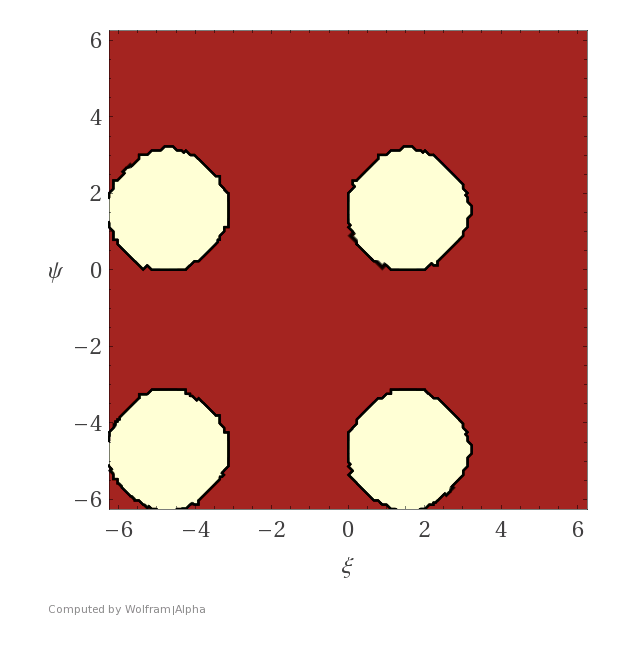
\includegraphics[height=8cm]{failurecase.png}
\caption{Imaginary components of $\sqrt{1-sin^{2}(\psi)-sin^{2}(\xi)}$.  The lightly shaded area are angles of pitch and roll that cause the failure of the zenith oriented solution.}
\label{f:failure}
\end{figure}
\begin{figure}[b!]
\centering
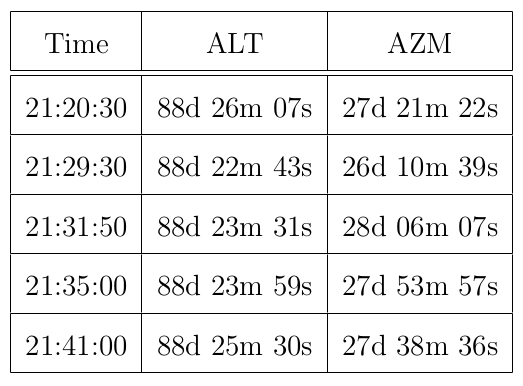
\includegraphics[height=4cm]{altitude.png}
\caption{Altitude (Zenith) Angle Orientation of CST}
\label{f:alt}
\end{figure}
\begin{figure}[b!]%2
\centering
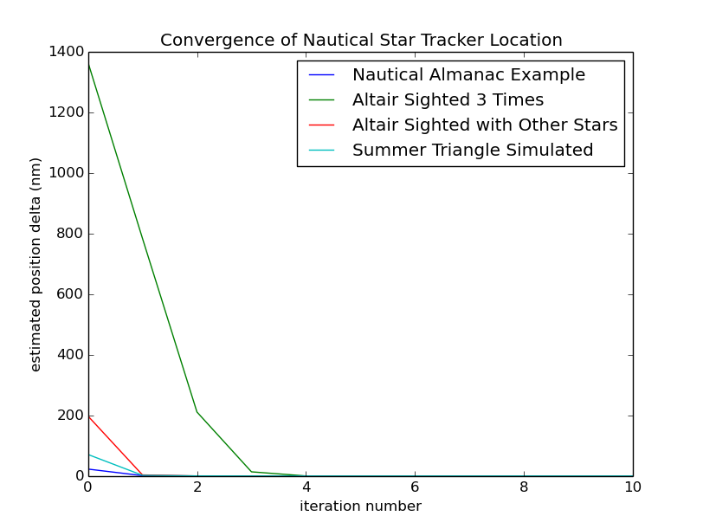
\includegraphics[height=8cm]{convergence.png}
\caption{Convergence of the different observational schemes.}
\label{f:converge}
\end{figure}
\begin{figure}[b!]
\centering
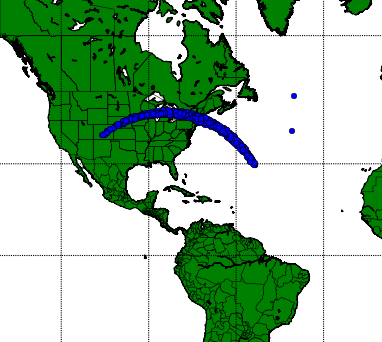
\includegraphics[height=8cm]{1s3t.png}
\caption{Position estimates for 1 star observed at 3 different times}
\label{f:1s3t}
\end{figure}
\begin{figure}[b!]
\centering
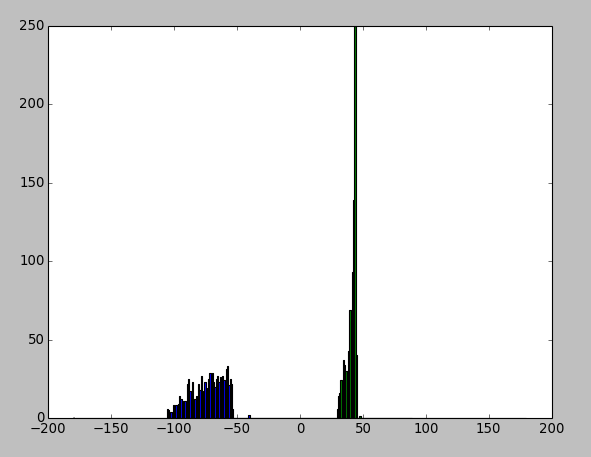
\includegraphics[height=8cm]{1s3t_hist.png}
\caption{Histogram of the positions for a single star observed at 3 different times}
\label{f:1s3t_hist}
\end{figure}
\begin{figure}[b!]
\centering
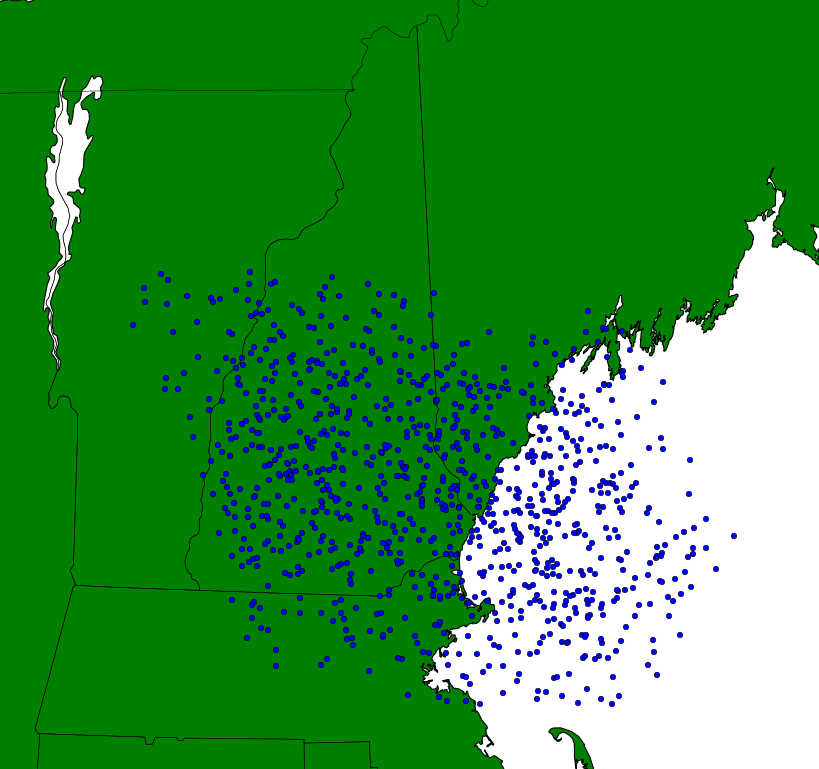
\includegraphics[height=8cm]{3s1t.png}
\caption{Position estimates for 3 stars observed at a single time}
\label{f:3s1t}
\end{figure}
\begin{figure}[b!]
\centering
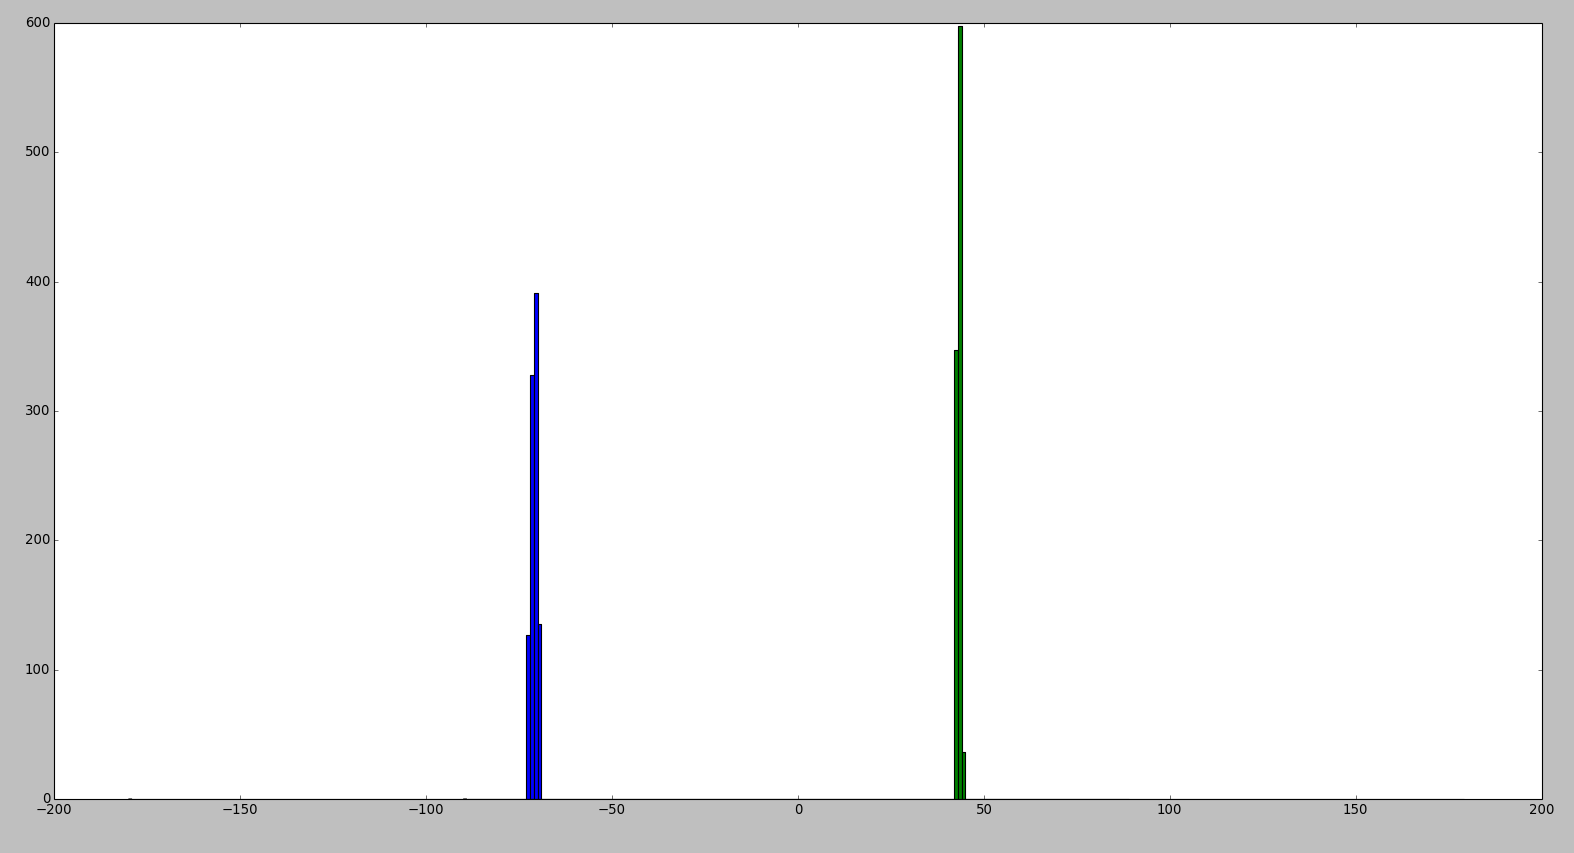
\includegraphics[height=8cm]{3s1t_hist.png}
\caption{Histogram of the positions for 3 stars observed at a single time.  In this image, the horizontal axis units are in degrees latitude or longitude.  The vertical is the frequency of each measurement, and the binning is one degree per bin.}
\label{f:3s1t_hist}
\end{figure}%6
\begin{figure}[b!]
\centering
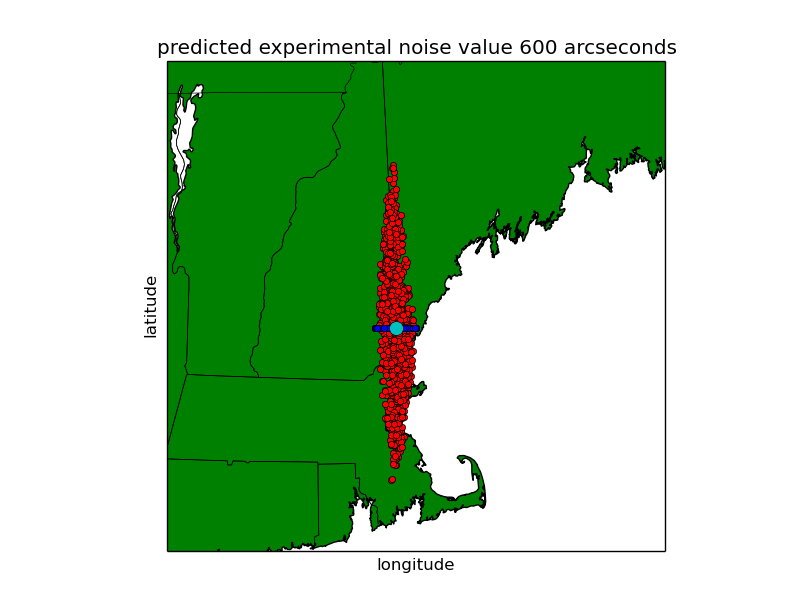
\includegraphics[height=8cm]{map2222.png}
\caption{Position estimates with 600 arcseconds uncertainty}
\label{f:crush}
\end{figure}
\begin{figure}[b!]
\centering
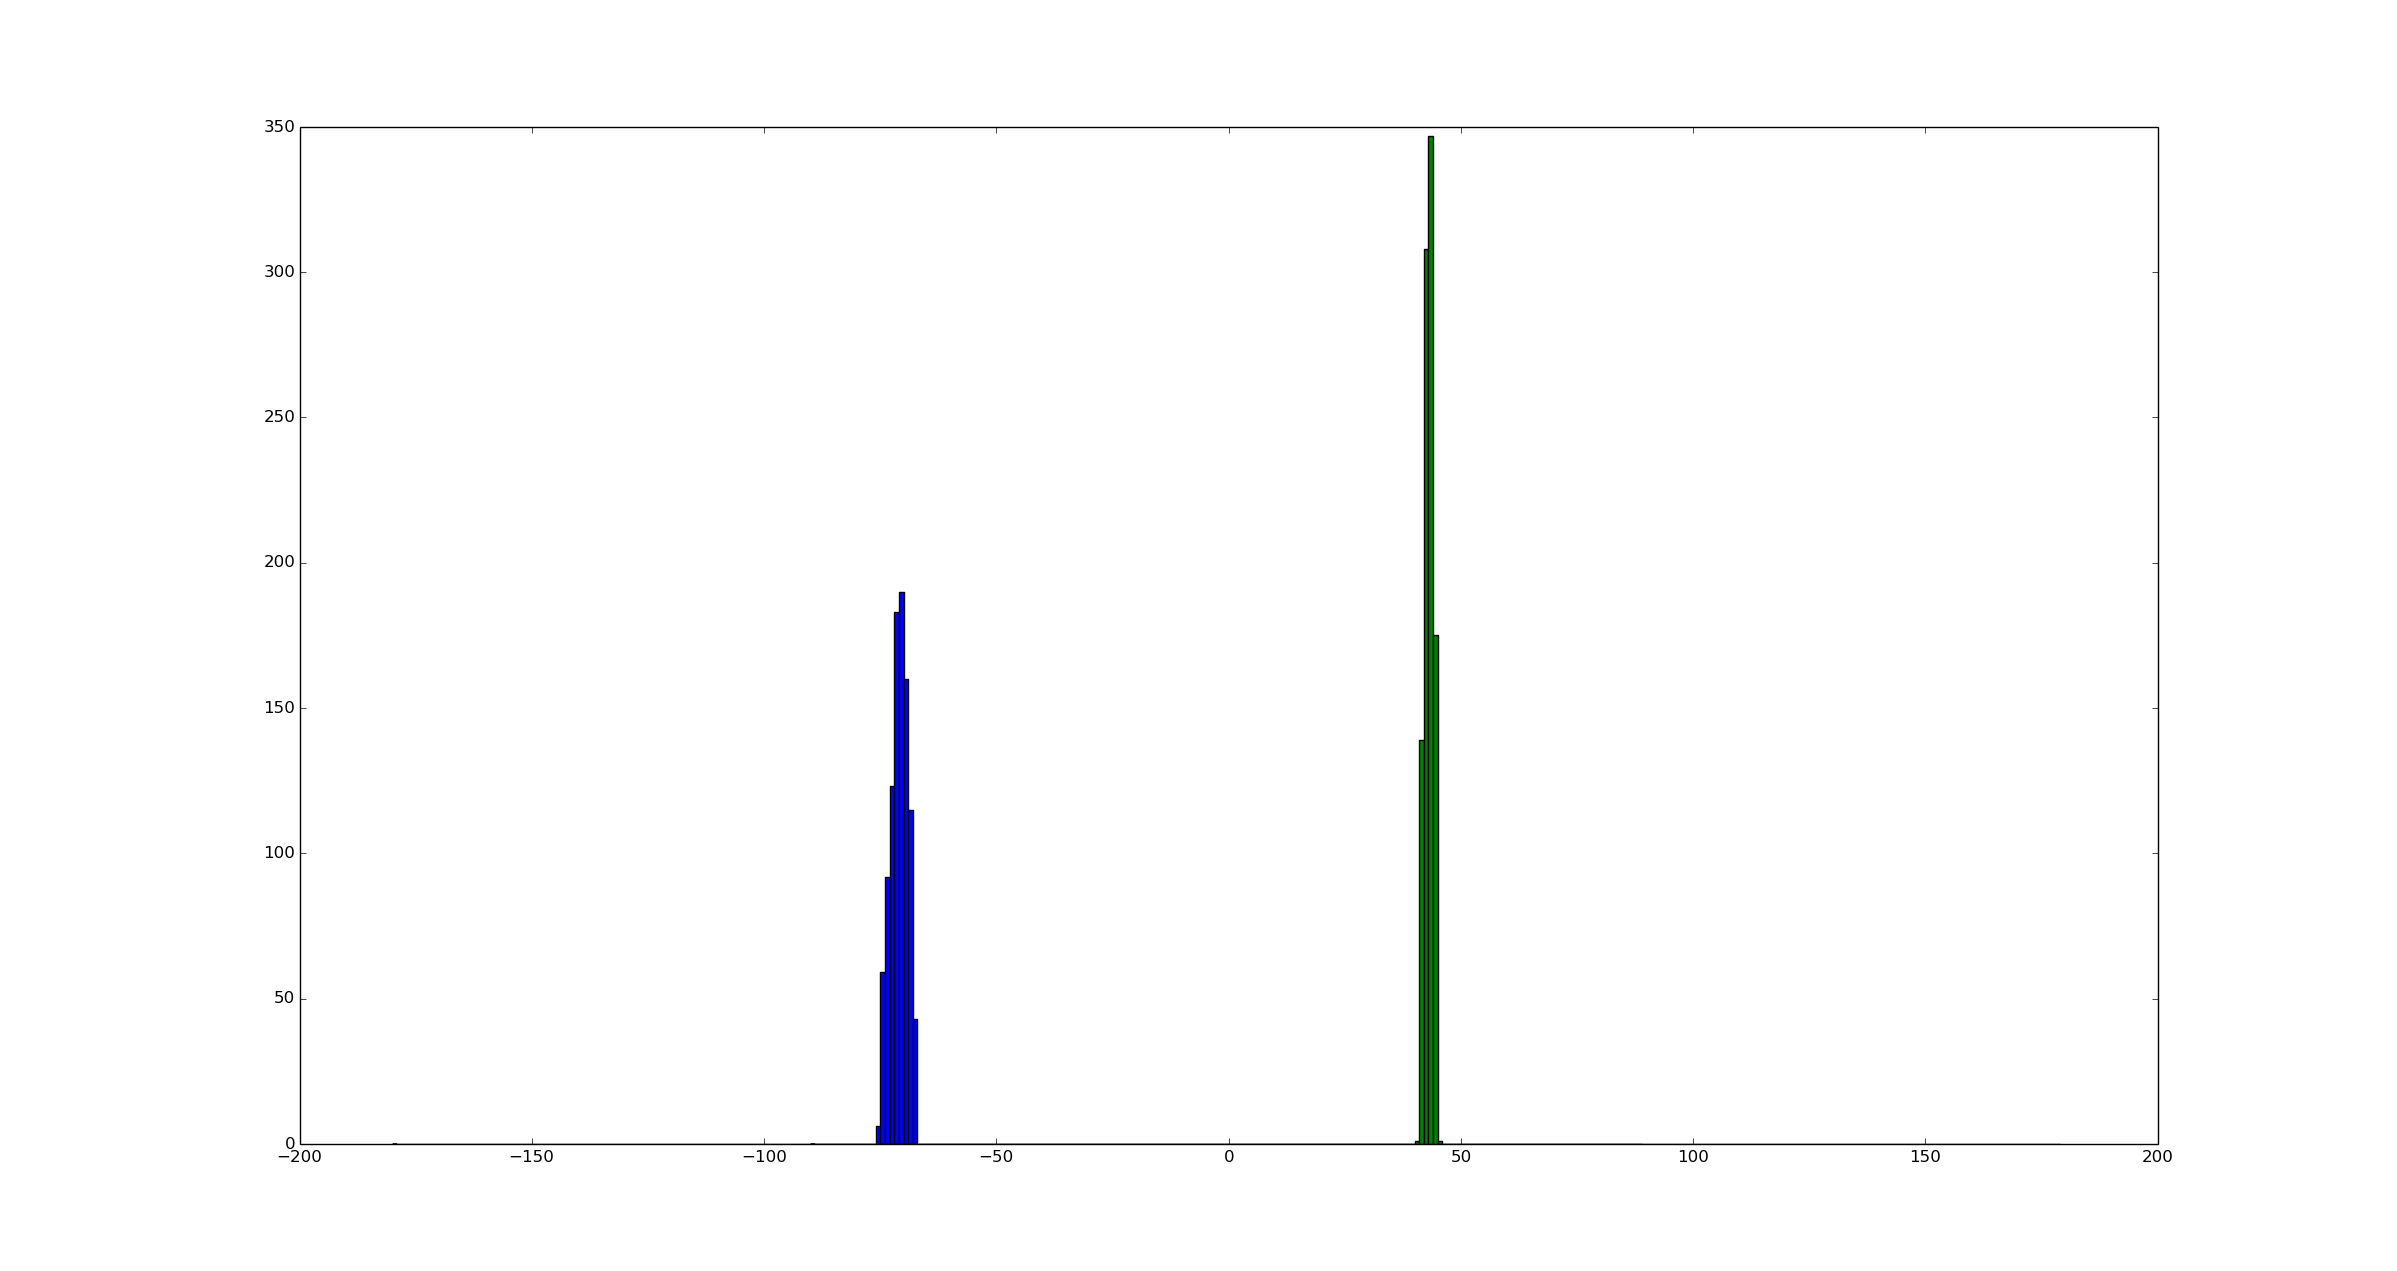
\includegraphics[height=8cm]{histogram2222.png}
\caption{Histogram of Latitude and Longitude (Degrees in the Domain, Frequency in the Range)}
\label{fig:hw2_prob1}
\end{figure}
\begin{figure}[b!]% order of placement preference: here, top, bottom
\centering
 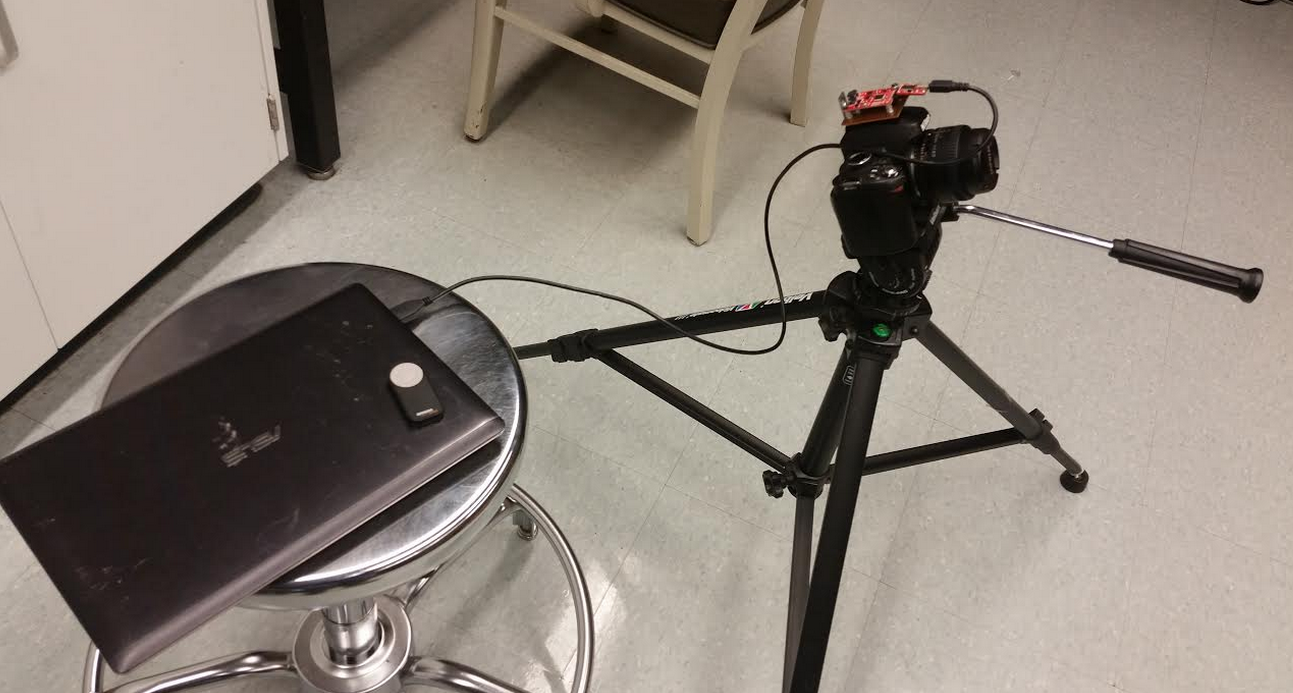
\includegraphics[height=8cm]{setup.png}
 \caption{Experimental setup for the Celestial Navigation Device.   The remote shutter can be seen on top of the laptop.}
 \label{f:setup}
\end{figure}
\begin{figure}[b!]
\centering
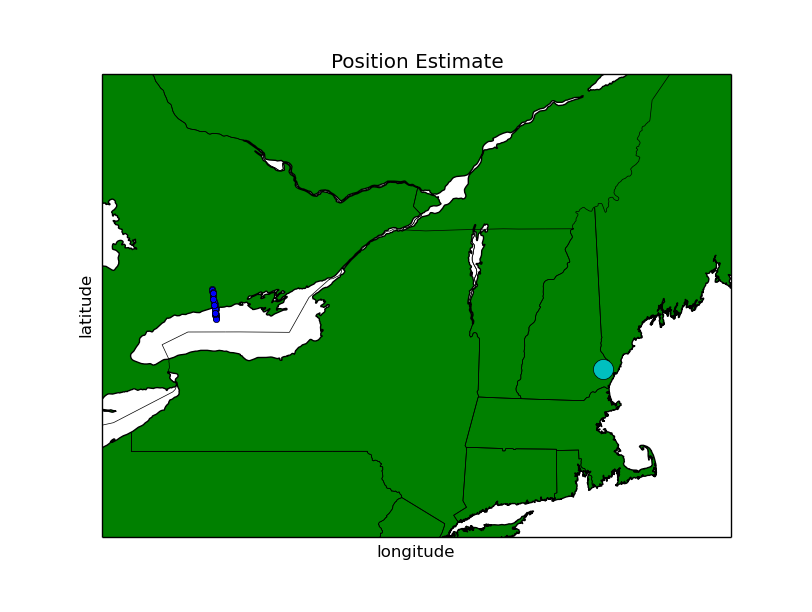
\includegraphics[height=8cm]{nomods.png}
\caption{Star Camera error with no modifications}
\label{f:nomods}
\end{figure}
\begin{figure}[b!]
\centering
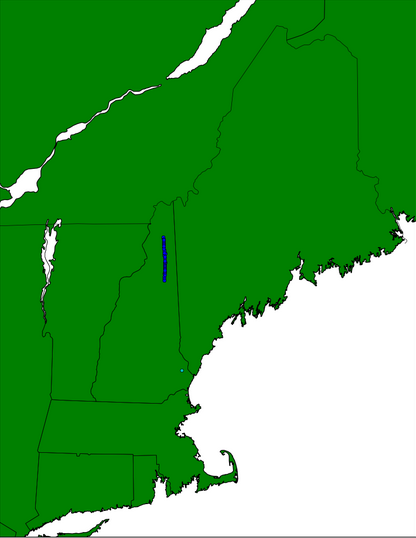
\includegraphics[height=8cm]{pitchmod.png}
\caption{Star Camera error with pitch modification}
\label{f:pitchmod}
\end{figure}
\begin{figure}[b!]
\centering
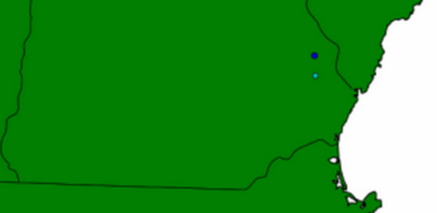
\includegraphics[height=4cm]{zrollmod.png}
\caption{Position estimate after roll modification}\label{f:zrollmod}
\end{figure}
\end{document}

% - Release $Name:  $ -
